%!TEX root = report.tex
When running the algorithm with a reasonable learning rate, \(\eta = 0.01\) and learning time \(t_{max} = 500\), the cost functions for both the training set and the test set are converging nicely.
This can be seen in Figure~\ref{fig:costs_t500_lr001}.
\myfigure{
	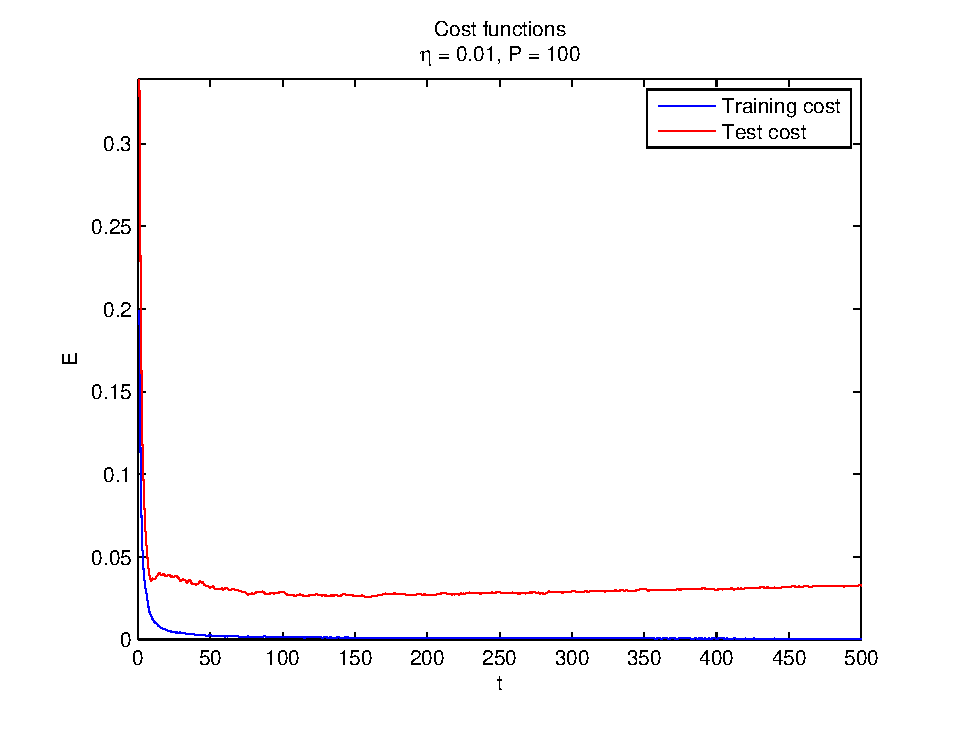
\includegraphics[width=\columnwidth]{costs_t500_lr001.eps}
	\figcaption{Cost functions using a reasonable learning rate and learning time}
	\label{fig:costs_t500_lr001}
}

When setting the learning time too large, a phenomenon called overfitting can be observed.
That is, the weights are highly optimized for the training set, but too specific to be reasonable for the test set as well.
The phenomenon is illustrated in Figure~\ref{fig:overfitting}.
\myfigure{
	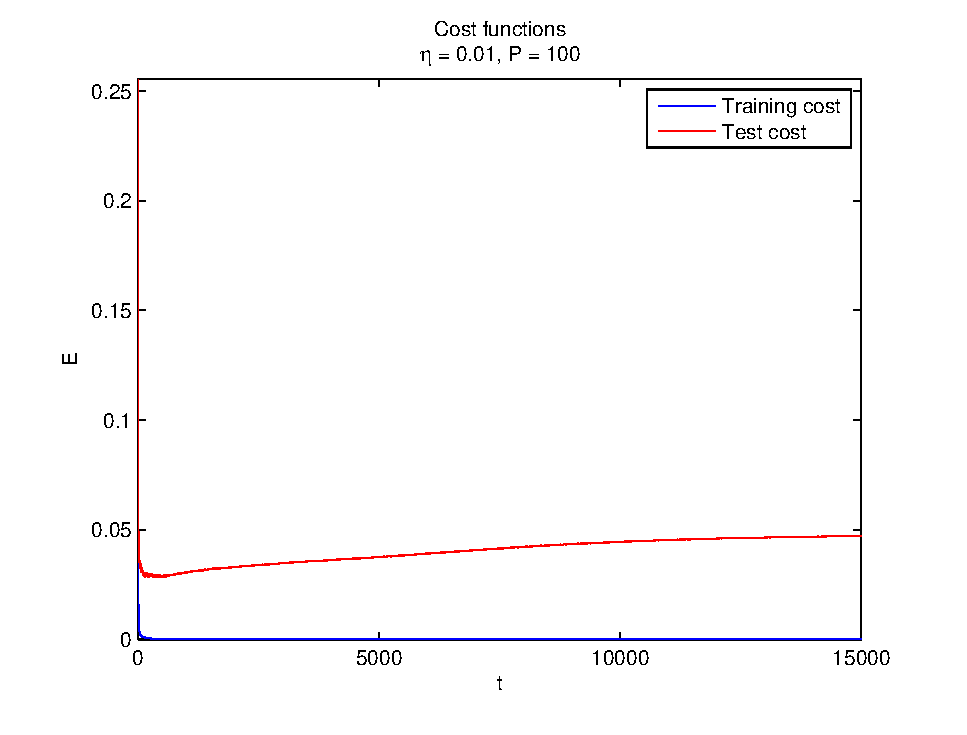
\includegraphics[width=\columnwidth]{overfitting.eps}
	\figcaption{When time progresses, the cost function for the training set keeps decreasing, but the cost function for the test set starts increasing at some point.}
	\label{fig:overfitting}
}

From the reasonable training in Figure~\ref{fig:costs_t500_lr001}, we've retrieved the weight vectors at \(t = t_{max}\), and visualized them using a bar graph in Figures~\ref{fig:w1_t500_lr001} and~\ref{fig:w2_t500_lr001}.
\myfigure{
	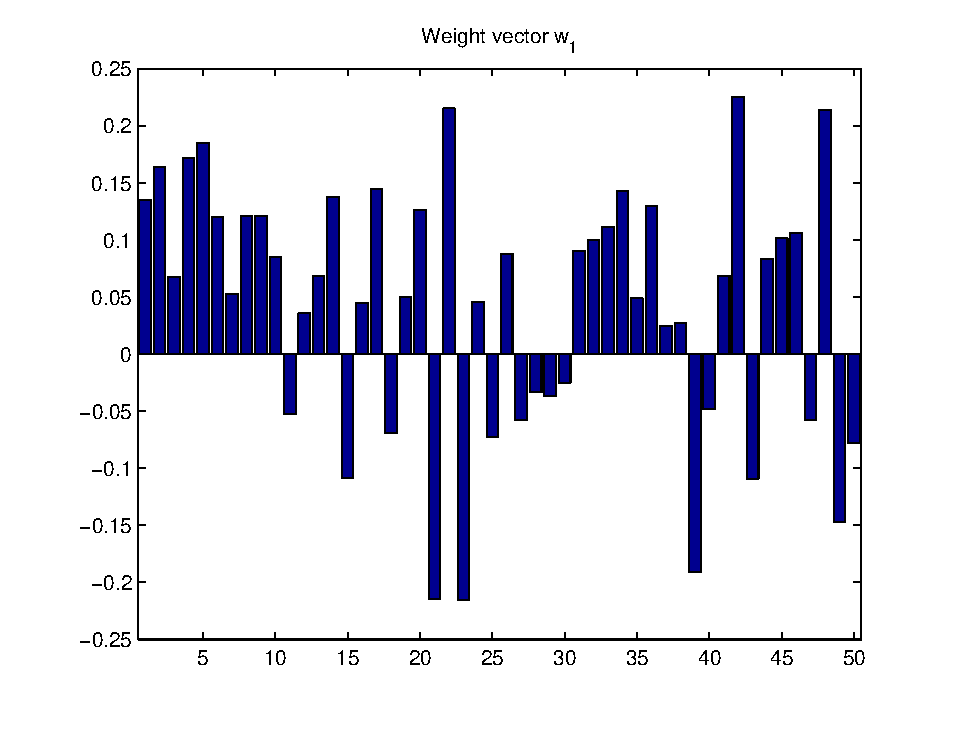
\includegraphics[width=\columnwidth]{w1_t500_lr001.eps}
	\figcaption{Visualization of \(w_1\).}
	\label{fig:w1_t500_lr001}
}

\myfigure{
	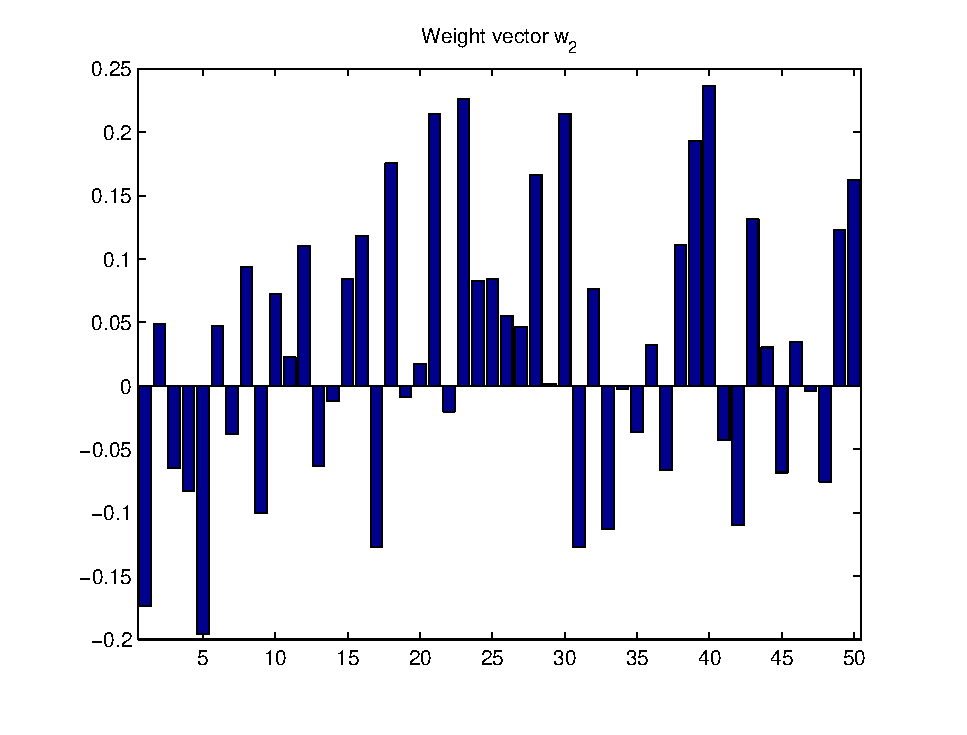
\includegraphics[width=\columnwidth]{w2_t500_lr001.eps}
	\figcaption{Visualization of \(w_2\).}
	\label{fig:w2_t500_lr001}
}